\section{Method}
In this section, we first describe our process of recruiting and remunerating participants, the brainstorming question selected for our experiments, and the user interface provided to workers. We then describe the data collected, and our method of organizing it into a hierarchical cluster for analysis.

\subsection{Recruitment and Remuneration}
We published brainstorming HITs (human intelligence tasks) on Amazon's Mechanical Turk. Workers were residents of the United States to increase the chances of English language comprehension and a shared cultural background.

HITs were placed on the marketplace asking for 5, 10, 20, 50, 75, 100, or as many possible ideas. HITs paid approximately 3.5 cents per idea requested, yielding reward amounts of 18 cents (5), 35 cents (10), 70 cents (20), \$1.75 (50), \$2.65 (75), and \$3.50 (100). For the unlimited condition, we offered \$1.75, pricing it the same as the 50 ideas condition. HITs were advertised with the number of responses requested. Workers had 18 hours to submit the HIT once accepted.

\subsection{Brainstorming Question: Uses for an Old MP3 Player}
In conducting this research, we tested several brainstorming questions, including classic brainstorming questions from prior work (e.g., ``provide alternative uses for a mop''); a request to brainstorm factors that influence weight gain and weight loss; and more goal-oriented questions, such as one requesting people to brainstorm ways to raise funds for a charity. Ultimately, we chose the goal-oriented brainstorming questions since they reflect what we believe would be real-world uses of brainstorming.

The final brainstorming question we chose is the following:
\begin{quote}
{\em Many people have old MP3 players or MP3 players that they no longer use. Please brainstorm N uses for old MP3 players/MP3 players. Assume that the devices' batteries no longer work, though they can be powered via external power sources. Also be aware that devices may {\em not \/} have displays. Be as specific as possible in your descriptions.\/}
\end{quote}


%This served as the independent variable in all data gathering. It must be stated that under normal brainstorming conditions, participants are asked to generate as many ideas as possible within a fixed time frame, instead of a fixed number. We excluded such a condition for two reasons. First, it is practice in crowd creativity tasks to solicit a fixed number of ideas (e.g. Yu and Nickerson \cite{yu_cooks_2011}). Secondly, we piloted asking respondants for "as many ideas as possible" in a generous time frame. Over N respondents, we received a mean of N ideas (std N), despite giving a financial of \$\$\$\$. This suggested a propensity to "game the system", a behaviour we wanted to exclude.

We focus on this problem because a) we expected workers to be familiar with problem area (old MP3 players), b) it represents a real-world problem (what to do with old electronics that are still partially functional), and c) we anticipated there to be a wide range of creative solutions possible. All data presented in this paper refer only to responses received to this particular question.

%Because workers could choose which \emph{number of ideas} condition to participate in, self-selection bias is a reasonable concern. However, this bias is also present in real-world HIT choice behaviour. 

\subsection{Worker's Brainstorming Interface}

Upon accepting a HIT, participants were asked to give consent for participating in the study, and informed that they could leave the study at any point without financial consequences. Under real-world conditions, workers would be expected to complete all responses to receive compensation.

The brainstorming task was presented in a standard web-based form that included the following components: an introduction, the specific brainstorming problem, a series of fields for entering the individual responses, and a larger text area where workers could enter additional ideas (Figure~\ref{fig:sample_task}).

\begin{figure}[h!]
    \centering
    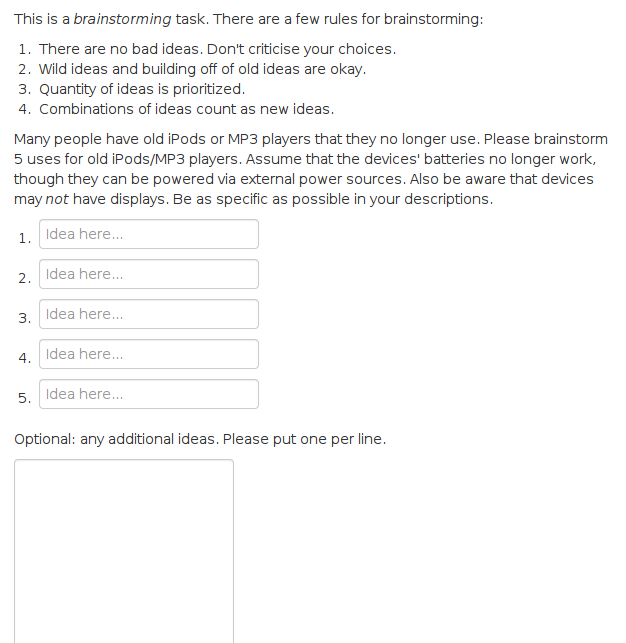
\includegraphics[width=0.9\columnwidth]{sample_task}
    \caption{Sample task on Mechanical Turk}
    \label{fig:sample_task}
\end{figure}

The introduction listed Osborne's four rules of brainstorming \cite{osborn_applied_1957}, adapted to this context.
%\begin{enumerate}
%\item There are no bad ideas. Don't criticise your choices.
%\item Wild ideas and building off of old ideas are okay.
%\item Quantity of ideas is prioritized.
%\item Combinations of ideas count as new ideas.
%\end{enumerate}
In addition to the visible text input fields, HITs were instrumented to collect the time of the first activation and last de-activation of each form element.

\subsection{Data Collected}

Initially, we sought 10 HIT responses per condition. However, we found that collecting only 10 responses for the lower response conditions (5, 10, 20 responses) limited our ability to make meaningful comparisons between responses received from the larger response conditions (50, 75, 100). Accordingly, we sought to collect a minimum of 400 ideas for each condition. However, we found the 5 and 10 conditions to be particularly unpopular, and were not able to reach this minimum for these conditions.

154 workers submitted 170 HITs, for a total of 3292 responses. As we received data in the unlimited condition, it became obvious that this was a poor strategy to employ -- the number of responses received was less than 15 in all cases. We remove that data from our analysis.

If a worker completed multiple HITs, there is the possibility that their responses and idea generation processes evolved over time. Only the first HIT submitted by each worker is retained.

We are left with 146 distinct participants for a total of 146 HITs, yielding 3007 responses. %A breakdown of responses across conditions is given in Table~\ref{tab:data_collected}.

%\begin{table}[h!]
%\begin{tabular}{r | l l l l l l l }
%    & 5 & 10 & 20 & 50 & 75 & 100 & all \\ \hline
%    participants & 57 & 39 & 21 & 9 & 10 & 10 & 146 \\
%    solutions & 283 & 372 & 413 & 450 & 635 & 855 & 3007
%\end{tabular}
%\caption{Data after removing unlimited condition and repeats}
%\label{tab:data_collected}
%\end{table}

%To uniquely identify participants, we computed a hash of their Mechanical Turk worker ID. A hash was used to protect privacy after data release.

\subsection{Hierarchical Clustering}
A significant challenge to creating model of brainstorming is efficiently identifying what ideas and categories of ideas are similar to one another. To address this problem, we organized the data into sets of hierarchical clusters, where parent nodes are more generalized versions of child nodes. %With this relationship, we are then able to calculate quantities such as the rate of novel ideas or novel idea categories, as a function of responses received. 

In the rest of this section, we introduce terminology useful for describing these hierarchical clusters, then describe the clusters and the process used to create them.

\subsubsection{Clustering: Terminology}
An \emph{instance} or \emph{response instance} is a single solution by a single participant to a brainstorming question. Most concretely, it is the text entered into a single field in the web form. For example, the following are four \emph{instances} from our data set:

\begin{enumerate}
    \item ``Storage Container"
    \item ``Small Storage Box"
    \item ``Coin Storage"
    \item ``Travel Jewelry Case"
\end{enumerate}

A \emph{brainstorming run}, or \emph{run}, is the temporally-ordered series of instances that were received in a single HIT.

An \emph{idea} is a unique solution to the brainstorming problem. An instance is associated with exactly one \emph{idea}, though multiple instances can be associated with the same idea. For example, in Figure~\ref{fig:example_instances}, we consider ``Storage Container'' and ``Small Storage Box'' as two instances of the same \emph{idea}. However, we do not consider ``Coin Storage'' to be the same idea, since it provides a more specific use case than the previous two. We use hierarchical clusters to encode these relationships. We call a hierarchical cluster of ideas a \emph{category tree}.

In a category tree, ideas act as nodes. Each idea may optionally have a single parent idea, and zero or more child ideas. If an idea \emph{A} is a parent of idea \emph{B}, A is a generalization of B. An example category tree for the instances above is given in Figure~\ref{fig:example_instances}.

\begin{figure}[!h]
    \centering
    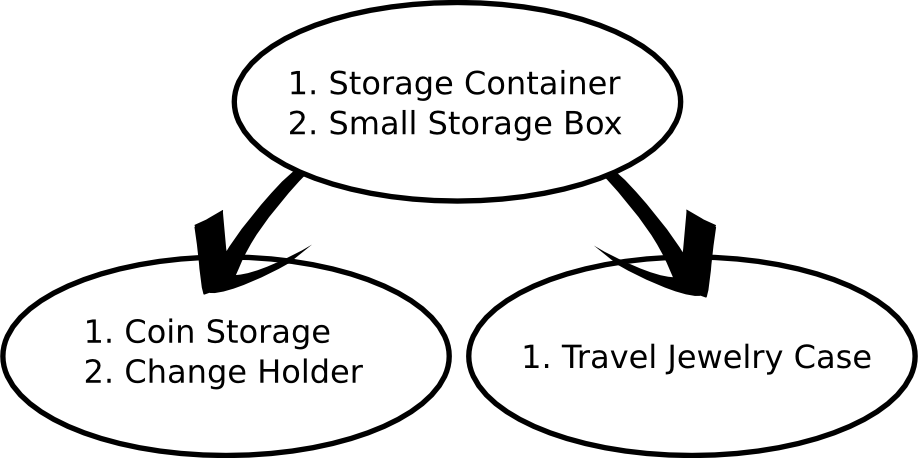
\includegraphics[width=0.9\columnwidth]{example_instances}
    \caption{Example category tree}
    \label{fig:example_instances}
\end{figure}

Category trees can either be \emph{singletons} or \emph{non-singletons}. A singleton category tree is composed of only one \emph{idea node}, the root. A non-singleton category tree has \emph{at least two idea nodes}. Non-singleton category trees correspond to the ``images'' described in Nisjstad and Stroebe's SIAM model \cite{nijstad_how_2006}.

Finally, the \emph{idea forest} is the collection of all category trees.

% \subsubsection{Clustering: Motivation}

% Initially, a coding scheme was employed in which a master list of unique ideas was formed, and each response was assigned a categorical code from this list. It proved difficult to determine and adhere to a constant granularity of distinction. For example, it is desireable to encode some equality between ``use [MP3 players] to build a chair, and "use [MP3 players] to build a table". Information loss results from either assigning both the same code or each different codes. An interval specificity scale is also difficult to employ; intuitively, we cannot compare the distance between ``audiobooks" and ``audio books for the blind" with the distance between the latter and ``[audio] instructions for the blind on a variety of things".

% A category tree allows the encoding of generalization relationships such that useful metrics can be extracted without any assumptions about distance.
% For example, The number of descendants of an idea gives a measure of how broadly that node was explored. 
% The prevalance of similar responses can be approximated at multiple levels; the number of instances under a tree represents the popularity of a category, while the same for an individual node provides a weighted score of ideas that are exactly equivalance.
% An idea can be considered more closely related to its adjacent ideas than it is to all other ideas in the tree.
% Using this common structure to operationalize originality and uniqueness ensures consistency in analysis. Furthermore, the category forest relies primarily on generalization decisions for construction, which are more clearly defined than equivalence.


\subsubsection{Clustering: Process}
To produce the idea forest, the primary author added instances to the idea forest using the following method.

If an instance described an idea already represented as a node in the forest, the instance was added to that node. Otherwise, a new node was produced.

If a node was a generalization of a second node, the second node was introduced as a child of the first. In some cases, two ideas were clearly related, though no generalization of the two existed in the data set. In these cases, we introduced a node that was a generalization of the two. For example, if we received only ``Coin Storage'' and ``Travel Jewelry Case'' as ideas, we would create a node labeled ``Storage Case'' to capture the fact that the two are related concepts. These ``artificial'' nodes were marked to distinguish them from true generalizations found in the data.

Clustering was performed using a custom-built tool that assisted in finding similar instances. The tool represented each instance using a query-expanded bag-of-words model ranked according to a cosine similarity metric.

The primary author clustered the 3007 response instances into ideas and category trees. A researcher not involved in the project randomly sampled 40 category trees to assess whether ideas within the tree should be there, and whether parent-child relationships correctly encoded generalizations of concepts. 10\% of the instances were marked as more specific than their associated idea, while 0.7\% of the instances were judged to be misclassified with their associated cluster tree.

\subsection{Data Analysis}
Throughout this paper, we employ Bayesian data analysis methods for modeling the data \cite{kruschke_doing_2010}. We express our results in terms of mean values and highest density intervals (HDI), or the interval that contains the most probable mass of the posterior distributions. In line with common practice, we choose an HDI of 95\%. To fit the models, we use the Bayesian inference software Stan \cite{stan-software:2013}, and choose uninformative priors for all modeled variables.

%In brief summary, the root idea that most closely matches the strategy in the instance is selected, and then that root idea and the new instance are compared in generality. This process may be repeated depending on this generality relationship, until instance is either placed in an existing idea or a new idea node is created.


% \begin{figure*}[ht]
% \small
% \begin{verbatim}
% for each instance:
%   idea_node = new node including instance
%   current_node = root of forest
%   do:
%     best_match = max_similarity(idea_node, current_node.children)

%     if best_match.similarity is low or current_node has no children:
%       insert idea_node under current_node
%       exit do
%     else:
%       if coverage(idea_node, best_match) == coverage(best_match, idea_node) == high:
%         merge idea_node, best_match
%         exit do
%       else if coverage(idea_node, best_match) == coverage(best_match, idea_node) == low:
%         new_parent = new artifical idea node
%         insert best_match, idea_node under new_parent
%         insert new_parent under current_node
%         exit do
%       else if coverage(idea_node, best_match) > coverage(best_match, idea_node):
%         replace best_match with idea_node in tree
%         current_node = idea_node
%         idea_node = best_match
%       else:
%         current_node = best_match
% \end{verbatim}
% \caption{Manual clustering algorithm}
% \label{fig:cluseringalg}
% \end{figure*}
